\scanpage{11}
\[
 \unsure{=|\Rightarrow}
\]
\[
 \mathbb P(X) \qquad
 P(X\times\unsure{Z|2})\overset{?}{\simeq}
 \operatorname{Hom}(\deleted{\unsure{e|\mathcal E}}Z\times X,\unsure{\mathscr E|\mathcal E})
\]
\[
 \mathrel{/\!/}\qquad
 \begin{tikzpicture}[baseline=(word.base),line cap=round,line join=round]
 % The first alternatives retain C's deletion annotation without adding a horizontal strike.
 % The cancellation target at the raised M/U and R remains uncertain.
 \node[anchor=base west,inner sep=0pt] (word) at (0,0)
 {$\rlap{$\operatorname{Hom}(X)$}\phantom{\deleted{\operatorname{Hom}(X)}}$};
 \node[inner sep=0pt] at (1.05,1.06)
 {$\unsure{\rlap{$M$}\phantom{\deleted{M}}|M|\rlap{$U$}\phantom{\deleted{U}}|U}$};
 \node[inner sep=0pt] at (1.72,.84)
 {$\rlap{$H$}\phantom{\deleted{H}}$};
 \node[inner sep=0pt] at (2.45,.95)
 {$\unsure{\rlap{$R$}\phantom{\deleted{R}}|R}$};
 \draw (-.06,.12) -- (2.14,.26);
 \draw (.02,.23) .. controls (.72,.26) and (1.76,.58) .. (2.45,1.03);
 \draw (.05,-.48) .. controls (.22,-.18) and (.73,.79) .. (1.03,1.09);
 \draw (1.28,-.52) -- (1.76,.94);
 \draw (1.57,.68) -- (1.87,.98) (1.58,.81) -- (1.85,.69);
 \draw[black!45] (.82,.28) -- (2.36,1.06);
 \node[inner sep=0pt] at (.02,.63) {\unsure{\begin{tikzpicture}[x=1cm,y=1cm]
 \fill (0,.02) -- (.04,0) -- (.035,-.025) -- (.005,-.01) -- cycle;
 \end{tikzpicture}}};
 \end{tikzpicture}
\]
\[
 \operatorname{Hom}(X,\underline{\operatorname{Hom}}(\mathscr E,Z)
\]
\[
 \unsure{O|0}\subset\mathbb P(X)\qquad
 \operatorname{Hom}(\mathscr E,\underline{\operatorname{Hom}}(X,Z))
\]
\[
 \begin{aligned}
 &\mathrel{/\!/}\\
 &P(\operatorname{Hom}(X,Z)
 \end{aligned}
\]
% crop-candidate: scan 11
\figure{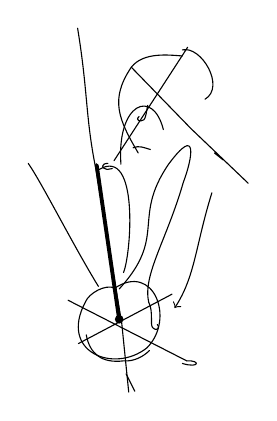
\begin{tikzpicture}[x=.011cm,y=-.011cm,line cap=round,line join=round]
\draw (63,1) .. controls (75,74) and (72,104) .. (84,163) -- (114,342) -- (122,421);
\draw[line width=1.4pt] (85,159) -- (111,337);
\draw (6,157) .. controls (22,180) and (57,250) .. (87,299);
\draw (64,365) -- (172,308) (52,315) -- (189,385);
\draw (106,301) .. controls (151,271) and (176,337) .. (143,370)
 .. controls (105,400) and (41,375) .. (72,317) .. controls (76,307) and (95,296) .. (106,301);
\fill (111,337) circle (5);
\draw (105,154) -- (190,23) (184,26) .. controls (206,21) and (234,69) .. (210,83)
 (125,46) -- (194,117) -- (260,180) (231,153) -- (221,145);
\draw (133,145) .. controls (110,106) and (100,83) .. (125,46) .. controls (139,28) and (169,32) .. (184,33);
\draw (113,158) .. controls (108,87) and (150,70) .. (162,118);
\draw (88,164) .. controls (134,137) and (125,261) .. (116,283);
\draw (111,302) .. controls (167,241) and (125,221) .. (168,158)
 .. controls (202,112) and (196,150) .. (185,179) .. controls (166,245) and (138,286) .. (145,317);
\draw[->] (218,191) .. controls (199,252) and (199,287) .. (175,324);
% Local small paths seen in the junction and disk crops; no letter or role assigned.
\draw (98,157) .. controls (90,157) and (90,163) .. (97,164) -- (103,163);
\draw (127,139) .. controls (134,136) and (140,139) .. (147,141);
\draw (144,90) .. controls (142,98) and (142,109) .. (136,108)
 .. controls (132,108) and (131,105) .. (134,103);
\draw (73,355) .. controls (77,377) and (91,388) .. (116,385)
 .. controls (128,386) and (139,380) .. (146,373);
\draw (189,385) .. controls (205,384) and (204,394) .. (184,388);
\draw (145,317) .. controls (151,329) and (146,344) .. (150,347)
 .. controls (156,352) and (158,345) .. (155,343);
\draw (119,400) -- (129,420);
\end{tikzpicture}}
\[
 \underline{\operatorname{Hom}}(X,Y)\subset P(X\times Y)
\]
\[
 \operatorname{Hom}(\overset{\text{\unsure{\begin{tikzpicture}[x=.07cm,y=.07cm,baseline=0pt,line cap=round]
 % Detached bent stroke and point above the overwritten lower Z; hand and role unsettled.
 \draw (0,0) -- (.45,.42) -- (.65,.13) -- (1.05,.35) -- (1.38,.26);
 \fill (1.68,.27) circle (.055);
 \end{tikzpicture}}}}{\deleted{\unsure{t|1}}Z}\times X,Y)\subset P(Z\times X\times Y)
\]
\diagram{\begin{tikzpicture}[x=.014cm,y=-.014cm,line cap=round,line join=round]
 % Coordinates below are the full scan coordinates minus (1150,380).
 % The displayed diagram retains all observed heads, the arch, and two unequal left rules.
 \node[inner sep=0pt] at (195,46) {$\rlap{$H$}\phantom{\deleted{H}}$};
 \draw[black!55] (160,68) -- (231,10);
 \draw (163,67) -- (183,54) (181,73) .. controls (183,82) and (204,68) .. (219,60);
 \draw (219,60) -- (227,109);
 \draw (163,101) .. controls (174,72) and (193,87) .. (198,112);
 \node[inner sep=0pt] at (67,139) {$\rlap{$\unsure{H|R}$}\phantom{\deleted{\unsure{H|R}}}$};
 \node[inner sep=0pt] at (83,143) {$P$};
 \node[inner sep=0pt] at (130,142) {$\rlap{$e$}\phantom{\deleted{e}}$};
 \node[inner sep=0pt] at (130,145) {$\times$};
 \node[inner sep=0pt] at (182,145) {$X$};
 \node[inner sep=0pt] at (214,151) {$\times$};
 \node[inner sep=0pt] at (254,145) {$Y$};
 \node[inner sep=0pt] at (294,148) {$\supset$};
 \node[inner sep=0pt] at (351,153) {$\rlap{$H$}\phantom{\deleted{H}}$};
 \node[inner sep=0pt] at (350,145) {$\Gamma$};
 % Overwriting strokes on the first factor and the heavy Gamma.
 \draw (62,120) -- (77,158) (61,146) -- (91,133);
 \draw[line width=1.2pt] (332,179) -- (333,123) -- (391,115);
 \draw (182,204) -- (177,264) (164,244) -- (177,264) -- (194,237);
 \node[inner sep=0pt] at (119,242)
 {$\rlap{$\unsure{H|U}$}\phantom{\deleted{\unsure{H|U}}}$};
 \draw (100,267) -- (141,191);
 \draw (127,255) .. controls (121,281) and (137,294) .. (151,272);
 \node[inner sep=0pt] at (155,246) {\unsure{\begin{tikzpicture}[x=.014cm,y=-.014cm]
 \fill (0,0) circle (1.6);
 \end{tikzpicture}}};
 \draw (319,193) -- (241,278) (247,250) -- (241,278) -- (266,270);
 \node[inner sep=0pt] at (176,326) {$P\times X$};
 \draw[line width=1.25pt] (161,364) -- (69,450);
 \draw (77,421) -- (69,450) -- (93,451);
 \draw (11,365) -- (9,565) (15,416) -- (25,551);
 \node[inner sep=0pt] at (39,513) {$P$};
 \node[inner sep=0pt] at (367,320) {$U\times_{\unsure{Y|V}}U$};
 \node[inner sep=0pt] at (195,447) {$\unsure{V|W}$};
 \node[inner sep=0pt] at (320,447) {$U$};
 \draw[line width=1.3pt] (291,446) -- (214,451);
 \draw (232,428) -- (214,451) -- (238,465);
 \draw (289,450) .. controls (267,457) and (237,458) .. (216,452);
 \draw (232,428) -- (236,419);
 \draw (190,498) -- (208,534);
 \draw[black!45] (291,487) -- (259,537);
 \fill (259,537) circle (1.2);
 \node[inner sep=0pt] at (230,595) {$P$};
\end{tikzpicture}}
% crop-candidate: scan 11
\figure{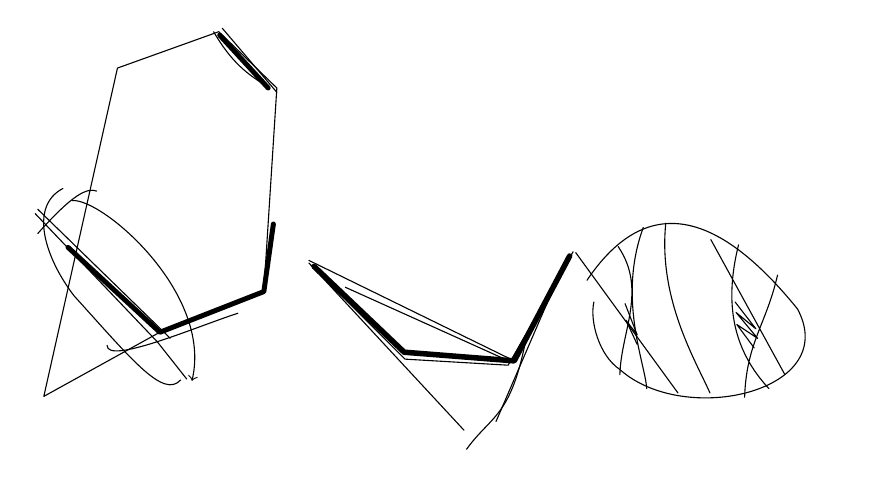
\begin{tikzpicture}[x=.011cm,y=-.011cm,line join=round,line cap=round]
\draw (13,425) -- (98,46) -- (215,4) -- (282,69) -- (267,303) -- (145,352) -- cycle;
\draw[line width=1.8pt] (216,8) -- (272,69) (278,226) -- (267,304) -- (147,351) -- (41,253);
\draw (209,4) .. controls (230,40) and (248,53) .. (272,68) (282,74) -- (219,0);
\draw (6,237) .. controls (47,191) and (63,184) .. (74,188)
 (3,214) -- (144,362) -- (178,405) (6,209) -- (159,358);
\draw (35,185) .. controls (-5,206) and (15,266) .. (48,309)
 .. controls (115,383) and (151,428) .. (171,406);
\draw[->] (46,199) .. controls (80,196) and (208,305) .. (184,407);
\draw (86,366) .. controls (86,389) and (188,345) .. (237,329);
\draw (319,271) -- (430,382) -- (549,389) -- (624,258) (319,271) -- (498,464) (535,454) -- (617,264);
\draw[line width=2pt] (325,275) -- (429,374) -- (556,384) -- (620,263);
\draw (319,268) -- (556,384) (361,299) -- (543,381);
\draw (501,486) .. controls (530,446) and (552,450) .. (570,357);
\draw (627,259) -- (745,421);
\draw (640,291) .. controls (722,169) and (814,239) .. (883,324)
 .. controls (934,419) and (753,461) .. (678,394) .. controls (654,378) and (643,338) .. (648,316);
\draw (676,252) .. controls (710,302) and (679,351) .. (678,400)
 (705,230) .. controls (675,312) and (707,386) .. (709,416)
 (731,225) .. controls (722,312) and (765,383) .. (782,421);
\draw (783,244) -- (868,399) (815,250) .. controls (797,322) and (811,374) .. (850,416)
 (860,285) .. controls (847,342) and (824,363) .. (822,426);
\draw (684,318) -- (698,354) -- (685,337) -- (698,365)
 (811,316) -- (835,347) -- (812,328) -- (837,358) -- (813,342) -- (833,369);
\end{tikzpicture}}
% archive sheet number: 10
